% arara: pdflatex: { interaction: batchmode }
\documentclass{article}
\thispagestyle{empty}
\usepackage[scale=.9,landscape]{geometry}
\usepackage{subcaption}
\usepackage{tikz}
\usetikzlibrary{
  knots,
  hobby,
  external,
  decorations.pathreplacing,
  shapes.geometric
}

\tikzset{
  external/figure name=knot,
  external/prefix=knotdiagrams/trefoil-,
  show curve controls/.style={
    postaction=decorate,
    decoration={show path construction,
      curveto code={
        \draw [blue, dashed]
        (\tikzinputsegmentfirst) -- (\tikzinputsegmentsupporta)
        node [at end, draw, solid, red, inner sep=2pt]{};
        \draw [blue, dashed]
        (\tikzinputsegmentsupportb) -- (\tikzinputsegmentlast)
        node [at start, draw, solid, red, inner sep=2pt]{}
        node [at end, fill, blue, ellipse, inner sep=2pt]{}
        ;
      }
    }
  },
  show curve endpoints/.style={
    postaction=decorate,
    decoration={show path construction,
      curveto code={
        \node [fill, blue, ellipse, inner sep=2pt] at (\tikzinputsegmentlast) {}
        ;
      }
    }
  }
}

\tikzexternalize

\let\origtikzsetnextfilename\tikzsetnextfilename
\def\tikzsetnextfilename#1{%
  \origtikzsetnextfilename{#1}%
  \mysetlabel{#1}%
}

\newcommand{\mysetlabel}[1]{%
  \gdef\mynextlabel{#1}}

\newcommand{\autolabel}{%
  \label{fig:\mynextlabel}
  \global\let\mynextlabel\relax
}


\tikzset{
  use Hobby shortcut,
  knot diagram/every strand/.append style={
    ultra thick,red
  },
  every picture/.style={
    execute at end picture={%
      \path ([shift={(-5pt,-5pt)}]current bounding box.south west)   ([shift={(5pt,5pt)}]current bounding box.north east);
    }
  }
}

\begin{document}
%\tikzset{external/force remake=true}

\begin{figure}
%% Trefoil
\subcaptionbox{Trefoil}[.25\linewidth][c]{%
  \tikzsetnextfilename{trefoil}
%\tikzset{external/export next=false}
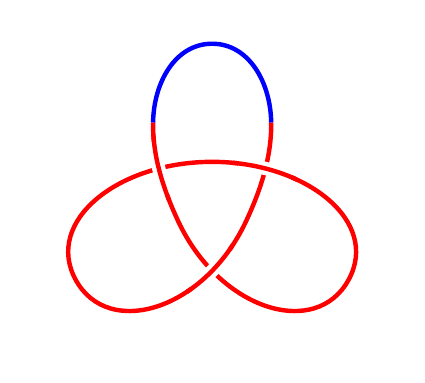
\begin{tikzpicture}
\begin{knot}[
  consider self intersections=true,
%  draft mode=crossings,
  flip crossing=2,
  only when rendering/.style={
%    show curve endpoints
  }
  ]
\strand ([closed,blank=soft]90:2) .. ([blank=soft]-.75,1) .. (210:.5) .. (330:2) .. (90:.5) .. (210:2) .. (330:.5) .. (.75,1);
\strand[blue,use previous Hobby path={disjoint,invert soft blanks}];
\end{knot}
\end{tikzpicture}
\autolabel
}%
%% Trefoil first twist
\subcaptionbox{Trefoil: First Twist}[.25\linewidth][c]{%
\tikzsetnextfilename{twist}
%\tikzset{external/export next=false}
\centering
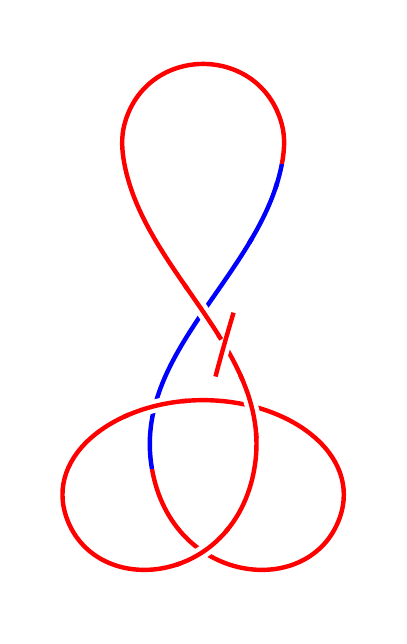
\begin{tikzpicture}
\begin{knot}[
  consider self intersections=true,
  end tolerance=3pt,
%  draft mode=crossings,
  flip crossing/.list={1,3,4}
  ]
\strand ([closed]1,4) .. (1,3.5) .. ([blank=soft]210:.75) .. (330:2) .. (90:.5) .. (210:2) .. (330:.75)  .. (-1,3.5) .. (-1,4);
\strand[blue,use previous Hobby path={invert soft blanks,disjoint}];
\end{knot}
\end{tikzpicture}
\autolabel
}%
%% Trefoil first move
\subcaptionbox{Trefoil: Move Over}[.25\linewidth][c]{%
\tikzsetnextfilename{first-over}
%\tikzset{external/export next=false}
\centering
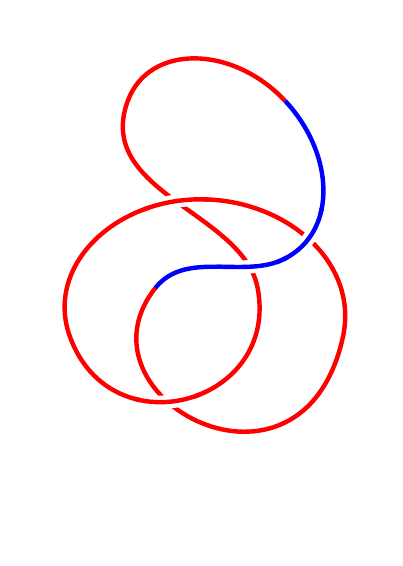
\begin{tikzpicture}
\begin{knot}[
  consider self intersections=true,
  end tolerance=3pt,
%  draft mode=crossings,
  flip crossing/.list={1,2,4}
  ]
\strand ([closed]1,2) .. ([blank=soft]1,0) .. ([blank=soft]210:.75) .. (330:2) .. (90:.75) .. (210:2) .. (330:.75)  .. (-1,2);
\strand[blue,use previous Hobby path={invert soft blanks,disjoint}];
\end{knot}
\end{tikzpicture}
\autolabel
}%
%% Trefoil slide round
\subcaptionbox{Trefoil: Slide Round}[.25\linewidth][c]{%
\tikzsetnextfilename{slide-round}
%\tikzset{external/export next=false}
\centering
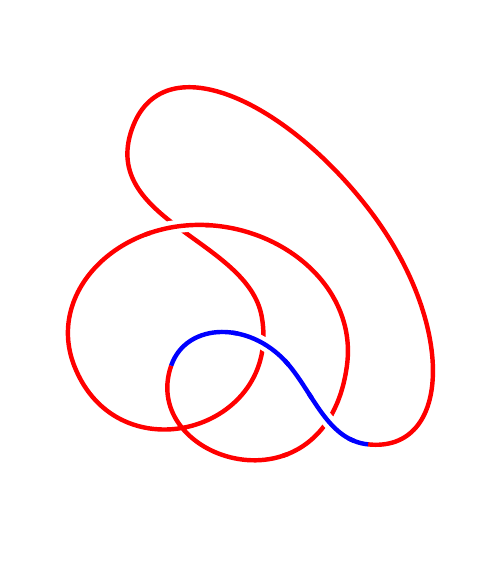
\begin{tikzpicture}
\begin{knot}[
  consider self intersections=true,
  end tolerance=3pt,
%  draft mode=crossings,
  flip crossing/.list={1,2,4},
  only when rendering/.style={
%    show curve endpoints
  }
  ]
\strand ([closed]2,1) .. (2,-2) .. ([blank=soft]1,-1) .. ([blank=soft]-.5,-1) .. (330:2) .. (0.25,.75) .. (210:2) .. (330:.75)  .. (-1,2);
\strand[blue,use previous Hobby path={invert soft blanks,disjoint}];
\end{knot}
\end{tikzpicture}
\autolabel
}
\end{figure}

\begin{figure}
%% Trefoil second move
\subcaptionbox{Trefoil: Second Move}[.25\linewidth][c]{%
\tikzsetnextfilename{second-move}
%\tikzset{external/export next=false}
\centering
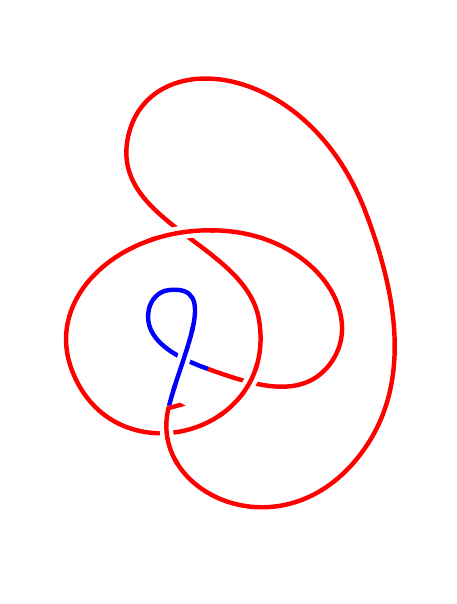
\begin{tikzpicture}
\begin{knot}[
  consider self intersections=true,
  end tolerance=3pt,
%  draft mode=crossings,
  flip crossing/.list={2},
  only when rendering/.style={
%    show curve endpoints
  }
  ]
\strand ([closed]2,1) .. (2,-2) .. (-.5,-1.5) .. ([blank=soft]-.5,0) .. ([blank=soft]-.75,-.25) .. ([blank=soft]0,-1) .. (1.5,-1) .. (0.25,.75) .. (210:2) .. (330:.75)  .. (-1,2);
\strand[blue,use previous Hobby path={invert soft blanks,disjoint}];
\end{knot}
\end{tikzpicture}
\autolabel
}%
%% Trefoil untwist
\subcaptionbox{Trefoil: Untwist}[.25\linewidth][c]{%
\tikzsetnextfilename{untwist}
%\tikzset{external/export next=false}
\centering
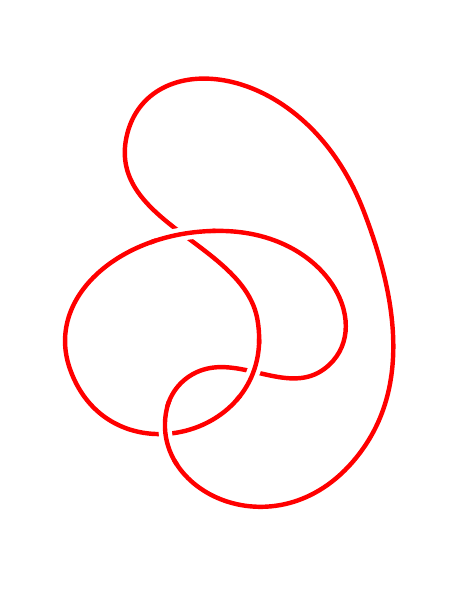
\begin{tikzpicture}
\begin{knot}[
  consider self intersections=true,
  end tolerance=3pt,
%  draft mode=crossings,
  flip crossing/.list={2},
  only when rendering/.style={
%    show curve endpoints
  }
  ]
\strand ([closed]2,1) .. (2,-2) .. (-.5,-1.5) .. (0,-1) .. (1.5,-1) .. (0.25,.75) .. (210:2) .. (330:.75)  .. (-1,2);
\end{knot}
\end{tikzpicture}
\autolabel
}%
%% Trefoil slide round
\subcaptionbox{Trefoil: Slide Round Again}[.25\linewidth][c]{%
\tikzsetnextfilename{slide-again}
%\tikzset{external/export next=false}
\centering
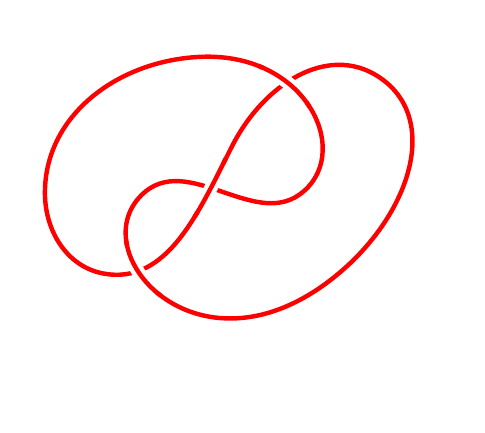
\begin{tikzpicture}
\begin{knot}[
  consider self intersections=true,
  end tolerance=3pt,
%  draft mode=crossings,
  flip crossing/.list={2},
  only when rendering/.style={
%    show curve endpoints
  }
  ]
\strand ([closed]2.5,.5) .. (2,-2) .. (-.5,-1) .. (1.5,-1) .. (0.25,.75) .. (210:2) .. (-1,-2) .. (330:.75);
\end{knot}
\end{tikzpicture}
\autolabel
}%
%% Trefoil neaten
\subcaptionbox{Trefoil: Neaten}[.25\linewidth][c]{%
\tikzsetnextfilename{neaten}
%\tikzset{external/export next=false}
\centering
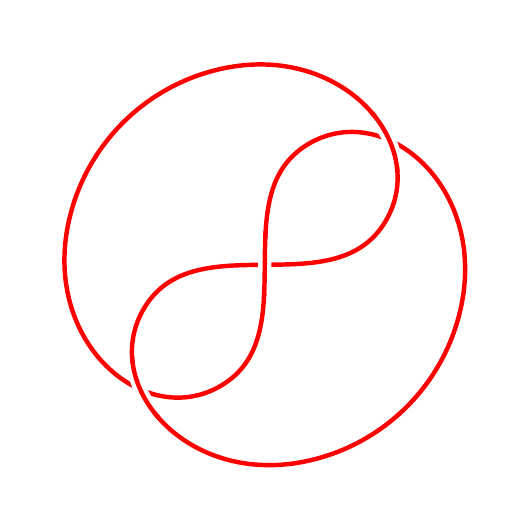
\begin{tikzpicture}
\begin{knot}[
  consider self intersections=true,
  end tolerance=3pt,
%  draft mode=crossings,
  flip crossing/.list={2},
  only when rendering/.style={
%    show curve endpoints
  }
  ]
\strand ([closed]0,2) .. (2,0) .. (-1,-1) .. (1,-3) .. (3,-1) .. (1,1) .. (0,-2) .. (-2,0);
\end{knot}
\end{tikzpicture}
\autolabel
}
\end{figure}

\end{document}
